\chapter{Prototype software application}
\label{chap:protype_software_application}

To empirically validate the feasibility of our proposed methodology, we developed a prototype application that implements the proposed configurations from the previous chapter.


\section{High-level architecture}

This application contains its frontend and its backend. The backend implements the generators and other services and provides them via an API. Users can use our frontend via a web application that communicates with the backend. On the backend, the LLM-assistant contains the following components:

\begin{itemize}
\item \emph{prompt manager} for fetching the prompt template based on the user input
\item \emph{RAG processor} for filtering a domain description based on the given class name
\item \emph{placeholder replacer} for replacing all placeholders in the prompt template with the input from the user
\item \emph{LLM manager} for sending the prompt to the LLM and parsing the output
\end{itemize}


\subsection{Work-flow}

On the frontend, through the user interface users can insert their input and then they can call some service provided by the backend. When the backend is called typically some generator is executed. First, the corresponding prompt template is retrieved by the \emph{prompt manager}. Then, all the prompt placeholders are replaced in the prompt template by the \emph{placeholder replacer}. For \emph{text to model generators} before the domain description is inserted, it can be filtered with some of the RAG technique by the \emph{RAG processor}. Subsequently, the assembled prompt is sent by the \emph{LLM manager} to the LLM and the output is parsed and optionally checked for mistakes. The approved output is then sent to the frontend and displayed to the user.


\begin{figure}[!h]
    \centering
    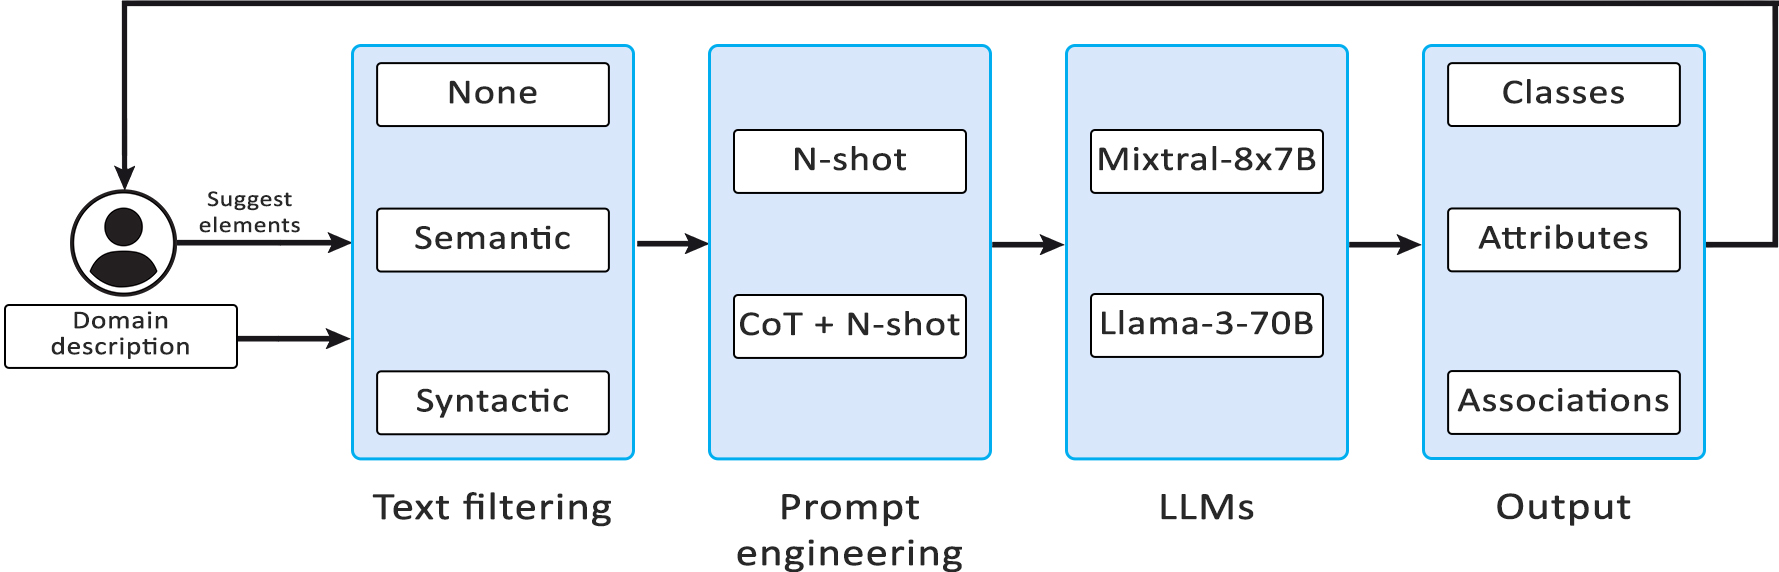
\includegraphics[scale=0.23]{img/work-flow.jpg}
    \caption{\centering Schema of the flow of processing the textual domain description}
    \label{fig:work-flow}
\end{figure}

Figure \ref{fig:work-flow} shows the basic flow of generating suggestions on the backend. The modeling process typically starts by providing the domain description. Then the domain model is step by step created mainly by using suggestions of classes, attributes, and associations from the assistant. Suggestions of attributes and associations are filtered by the selected retrieval-augmentation generation method. Then the prompt engineering techniques are applied and the final prompt is constructed and sent to LLM. Finally, the output from the LLM is parsed and the suggested model elements are sent back to the frontend. \\

\noindent{}TODO: Tady před obrázkem a po obrázku říkám skoro to samé, takže by se to hodilo nějak spojit.


\section{Assistant features}

The frontend web application contains a text area for inserting a domain description and a modeling canvas where the users create the domain models using classical manual modeling features and the suggestion features highlighted by the \textit{magic wand} icon.

Our LLM-based assistant provides the following services:

\begin{enumerate}
\item suggesting domain elements
\item highlighting already modeled elements
\item summarizing domain model
\end{enumerate}


\subsection{Suggesting domain elements}

When a domain description is provided, the assistant generates suggestions solely based on the provided text. Otherwise, the assistant does not adhere to any text. Our assistant can suggest classes. For a selected class the assistant provides functionality to suggest its attributes and associations. Also, for a selected source class and a selected target class, the assistant can suggest their associations. Figure \ref{fig:assistant-features} demonstrates some of these features.

\begin{figure}[!h]
    \centering
    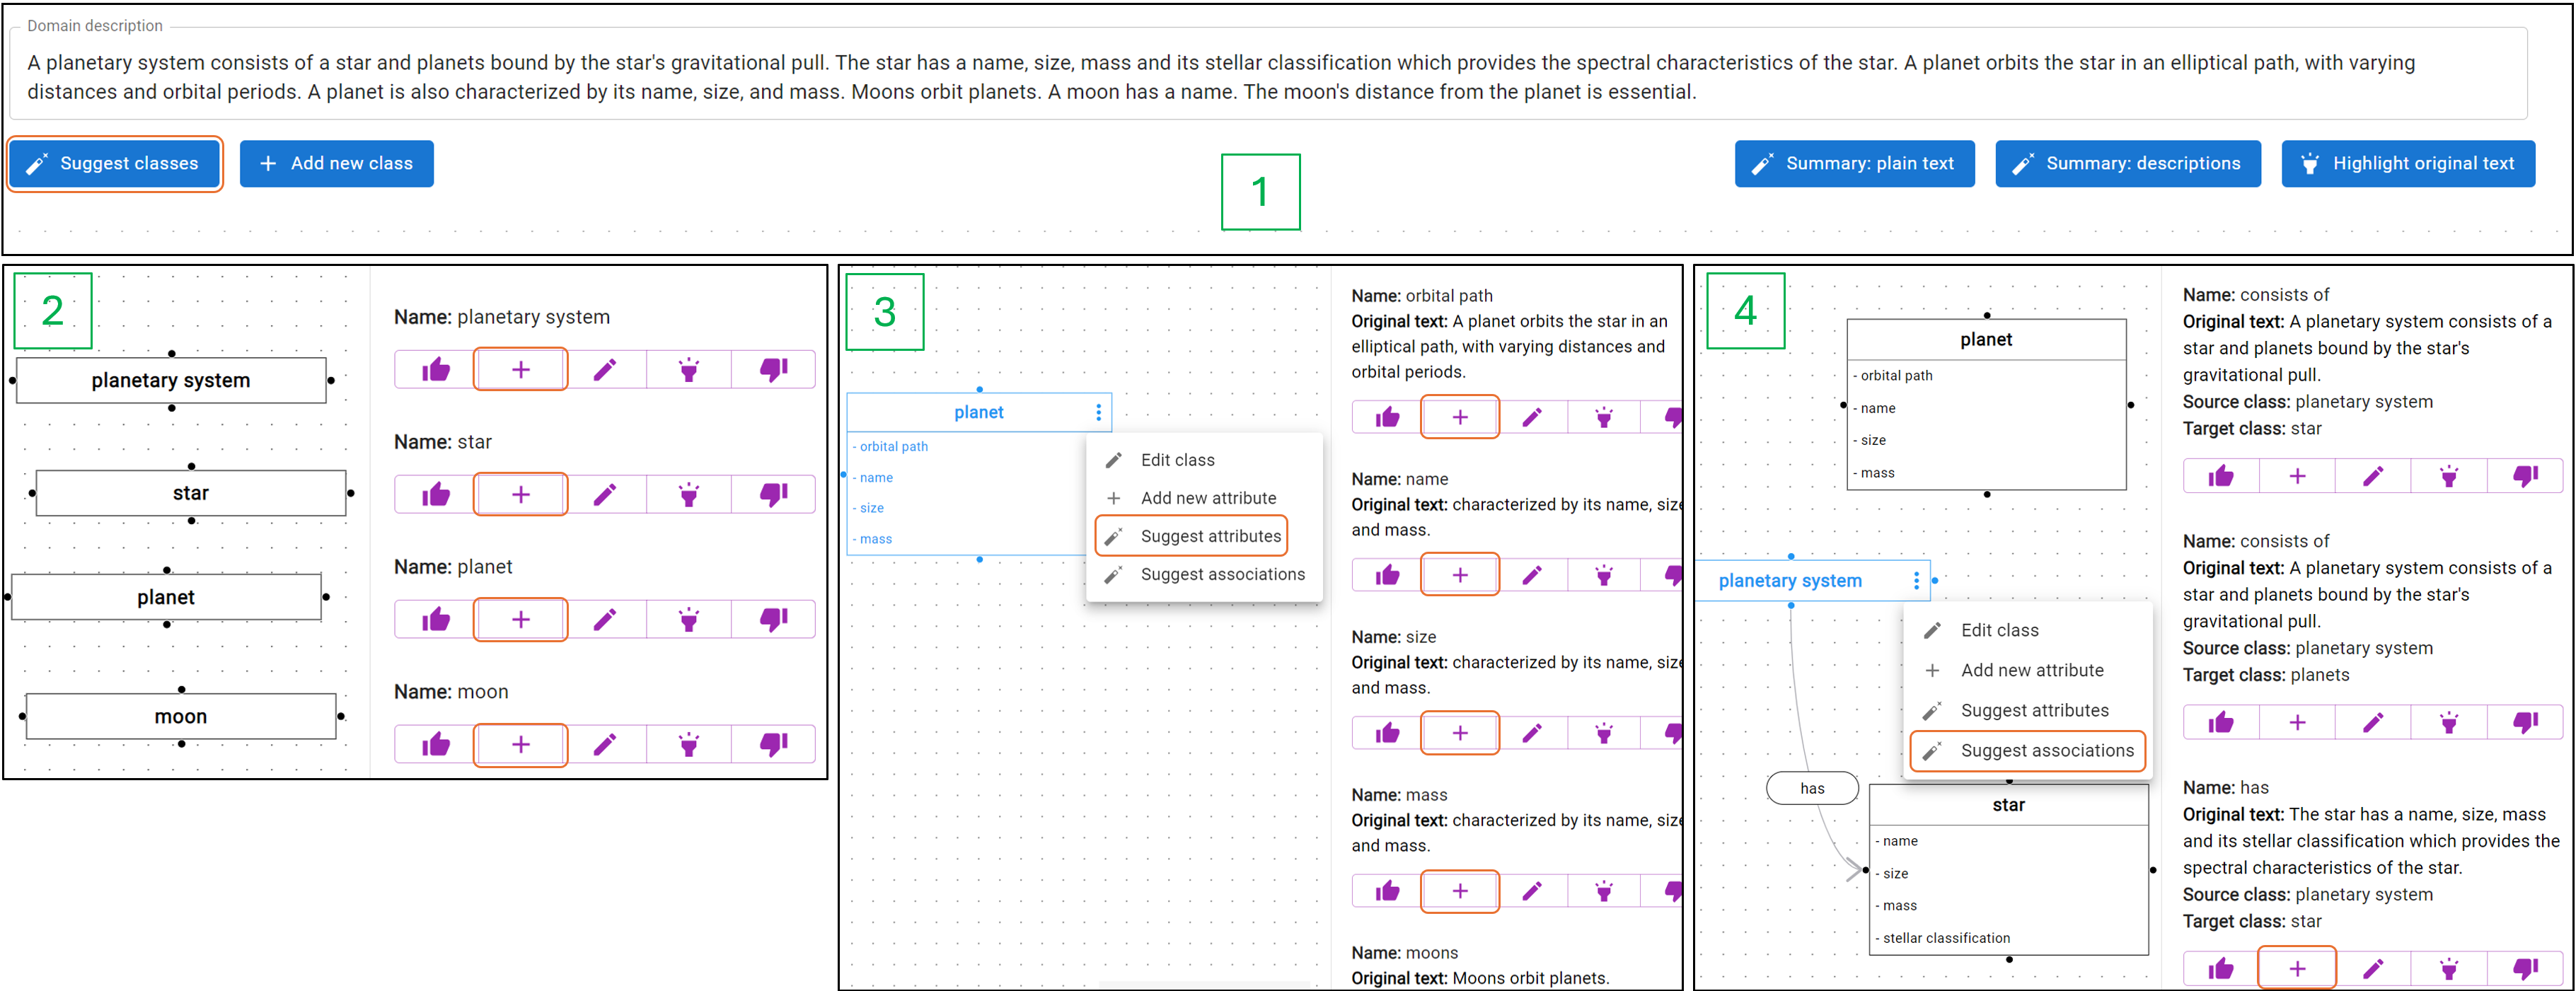
\includegraphics[scale=0.22]{img/assistant-features.png}
    \caption{\centering Screenshots of the main functionalities of the prototype application}
    \label{fig:assistant-features}
\end{figure}

Screenshot 1 shows the text area for the domain description and the action buttons. The highlighted button \textit{Suggest classes} calls the $gen_c$ operator with the inserted domain description. Screenshot 2 shows the list of suggested classes. The user can use the highlighted ``\textit{+}'' buttons to insert suggested classes into the modeling canvas. The other buttons are used for \textit{liking} and \textit{disliking} the corresponding suggestion, for editing before inserting the suggested class into the canvas, and highlighting the suggestion in the original domain description. For the selected class, the user can ask for attribute and association suggestions, i.e. $gen_a$ and $gen_{r1}$ operators for the class and the domain description. Screenshot 3 shows the attribute suggestions. Screenshot 4 shows the association suggestions. For the suggested attributes and association, the tool also shows the original text returned by the operators $gen_a$, $gen_{r1}$ and $gen_{r2}$.


\subsubsection{Context highlighting}
\label{sec:context_highlighting}

As mentioned, for each suggested attribute and association we highlight its original text in the domain description. Additionally, for each class, we highlight its name. This requires matching the LLM-generated original text with the domain description. The matching is easy as long as the original text syntactically exactly matches some part of the domain description.

However, we encountered some common issues with this approach. For example, sometimes the LLM changes some letters when generating the original text. For instance, when the domain description contains the word ``\textit{motorized}'' with the ``\textit{z}'' letter the LLM can generate the word ``\textit{motorised}'' with the ``\textit{s}'' letter instead.

To mitigate this issue we implemented the following recovery strategy. When the original text and the domain description cannot be directly matched we find their longest common substring and we split the original text into the longest common substring and the remaining parts. Subsequently, we try to match these parts without the letter that was in between these parts. For example, consider the original text that contains the word ``\textit{motorized}'' and the domain description that contains the word ``\textit{motorised}''. Let's assume that their longest common substring is the word ``\textit{motori}'' and the remaining common part is the ``{\textit{ed}}''. Subsequently, we find all occurrences of the word ``\textit{motori}'' in the domain description, and for each occurrence we then try to match the remaining part ``\textit{ed}''. In more complex scenarios this recovery strategy can fail however, this issue can be greatly mitigated by using a LLM with a high performance.


\subsubsection{Single field suggestion}

For the best possible LLM output quality and response time when generating suggestions, we try to simplify the prompts as much as possible. This for example means that the generated suggestions of attributes do not contain the attribute description or the attribute data type. For generating these additional fields our assistant can be used as it implements the generators for suggesting descriptions, data types, and cardinalities. Furthermore, if the generated domain element name is not suitable it can be re-generated by the generator for name suggestions.


\subsubsection{Attributes and associations conversion}
\label{sec:attributes_and_associations_conversion}
Attributes can be usually modeled as associations and vice versa. For example, \textit{address} can be an attribute of a class \textit{person} but it also can be an association between the classes \textit{person} and \textit{address}. Therefore, for each attribute suggestion, we provide functionality to convert them to an association and vice versa. We convert an attribute into an association by putting the attribute name into the association target class and we put the attribute name into the association name. As the copied name does not have to fit, the LLM assistant can be used to generate a new name. The opposite conversion from an association to an attribute works the same but in reverse.


\subsubsection{Duplicate domain elements}
\label{duplicate_domain_elements}

The generated domain element suggestion is not shown to the users if they already modeled the corresponding element. We remove these suggestions on the backend after the LLM generates the output so we do not have to provide the user's domain model in the prompts for generating classes, attributes, and associations.

The domain element suggestion is removed if its name syntactically matches the name of the user's corresponding modeled element. This approach has the following limitations.

The first limitation is that if two domain elements have the same name but different semantics then a relevant domain element is removed. For example, the class \textit{car} can have an attribute \textit{year} referring to the year of the car manufacturing and the same attribute referring to the year of the last technical inspection. In our experience, this issue is very rare as the LLM usually generates suggestions with explicit names so in this case the first mentioned attribute would probably be named \textit{year of manufacturing} and the second attribute would probably be named \textit{year of technical inspection}.

The second limitation is that the semantically same domain elements with a different name are not removed. Possible solutions are to either use an LLM or some embedding model as in our RAG semantic approach. However, both have significant disadvantages. Solving the mentioned problem with an LLM in a single prompt approach complicates the prompt wording and can reduce the output quality. Using LLM in an iterative prompt approach can significantly increase the delay between the user's request and showing the corresponding suggestion as the LLM has to process more than one prompt. When using some embedding model as mentioned in the section \ref{sec:top_k_search}, one of the challenging tasks is setting the threshold of the decision boundary between accepting and rejecting the corresponding element. For example, attributes \textit{first name} and \textit{last name} are very close in terms of vector space distance however, they represent two semantically distinct different attributes. This fact would force us to set a very strict threshold that would reject almost any two syntactically different words which is as a result almost identical to our naive approach.


\subsection{Highlighting already modeled elements}

We extend the mentioned highlighting of suggested domain elements in the domain description by highlighting all the selected user's modeled elements in the domain description. However, these highlighted parts do not have to always correspond with the parts that the user has already modeled as we only instruct the LLM to generate the context for each attribute and association. This means that this context can contain other classes, attributes, or associations. Consider the following example: \\

\noindent{} ``\textit{A person is identified by an ID card or by a driving license.}'' \\

\noindent{} When the LLM suggests the attribute \textit{ID card} its original text can contain also the \textit{driving license} that can be also modeled as an attribute.

Also, the not highlighted parts of the domain description can also be already covered by the user's domain model for example, if these parts were modeled manually by the user. This case can be solved by using the original text generator.


\subsection{Summarizing domain model}
\label{summarising_domain_model}

For a selected part of the user's domain model, the assistant is able to generate a summary for each class, attribute, and association using the \emph{summary generators}.

The summary plain text generator outputs a paragraph describing the selected part of the domain model in a given style. The summary style can be changed in the settings. The available styles are \textit{analytical}, \textit{educational} and \textit{funny story}. Before the summary is generated, the selected style is inserted into the corresponding prompt template in the \emph{modeling procedure}. The summary descriptions generator outputs a list where each selected domain element corresponds to one described item in the list. In both cases, the LLM does not receive the user's domain description as this led to many situations where the LLM did not stick to the selected domain elements.


\section{LLM parameters}

For each task, we set the temperature to the lowest value so the LLM generates only the most probable output as discussed in the section \ref{temperature}. For generating the summary, the temperature could be set higher to provide more creative output.

The other parameters are implicitly set to their default values which are defined in the OpenAI API\footnote{\url{https://platform.openai.com/docs/api-reference/introduction}}.


\section{LLM output checking}

When LLM generates any JSON object we always automatically remove those objects that do not contain all mandatory fields such as the name when generating classes, attributes, and associations. When the generated domain element is an association then we also remove the associations with a source class or a target class that does not match the user input. Additionally, as mentioned in the section \ref{duplicate_domain_elements}, the generated domain element is removed if it is already present in the user's domain model.


\section{Saving users data}

For each generated suggestion users can optionally click on the \textit{like} button or the \textit{dislike} button. The corresponding evaluated suggestion is sent to the backend and saved there with all the parameters that were used to generate this suggestion. To remember these parameters, the frontend remembers for each suggestion the parameters that were used for generating this suggestion.

We use these user's reactions for two main reasons. The first reason is that we can use these data as feedback. For example, we could automatically detect if some set of parameters repeatedly ended up with too many negative reactions. After that, we can analyze the issue and fix it. The second reason is that we can use these data for fine-tuning some LLM to further improve the quality of our specific tasks.

The downside of our approach is that it does not collect much user data. One possible solution is to save each user action such as saving each suggestion that the user added into his domain model. However, this approach has a lot of disadvantages. For example, if the user adds some suggestion and then later on removes it we need to save this removal action too as it can mean that the original suggestion turned out to be unwanted. This means that the saved data would need to be post-processed to remove these pairs of data. A similar issue arises when a user adds some suggestion but then later on edits it. Because of this complexity, we decided to use the explicit reactions buttons.


\section{Retrieval-augmented generation}
\label{sec:rag_implementation}

Now we describe the implementation of our semantic and syntactic RAG approaches and we present the most significant challenges we encountered when implementing them.


\subsubsection{Domain description segmentation}

Determining the chunk size is a challenging task since with too big chunks we risk having irrelevant parts of domain description in the prompt and thus decreasing the LLM performance. On the other hand, with too small chunks we risk that the chunks will be miss-classified as they will not contain enough information about their context to decide if they are relevant.

As a result, we consider each sentence of the domain description as one chunk since one sentence usually contains information about one concept or a few related concepts. The advantage of this approach is that after the chunks evaluation is done it is easy to concatenate the relevant chunks together simply by putting them next to each other in the original order from the domain description. On the other hand, the disadvantage is that for example, if some sentence refers to another sentence with a pronoun then without any additional domain description pre-processing this context is lost after the domain description segmentation.


\subsubsection{Lack of context}

As mentioned, chunks in the form of isolated sentences can be miss-classified if not enough context is provided. This mostly happens when some sentences contains pronouns that refer to some other sentences. For example, consider the class named \textit{book} and the following domain description: \\

\noindent{}``\textit{The book contains a lot of pages. It is very heavy.}'' \\

\noindent{}Now when classifying the chunk ``\textit{It is very heavy.}'' it most likely will be classified as an irrelevant chunk as in isolation it does not contain any information about the class \textit{book} even though the attribute \textit{weight} of the \textit{book} could be inferred from it.

To solve this issue and similar issues, we implemented a simple naive algorithm where each chunk has its metadata, and if a chunk starts with a pronoun we insert in its metadata the previous chunk. Now when a chunk is being evaluated, its metadata are also considered. This means that when classifying the second chunk from the example also the first chunk is present therefore the context is not lost. The disadvantages of this approach are that pronouns that are not at the start of a chunk are not considered. Also, adding a whole previous chunk to a current chunk can in some cases lead to miss-classification if the current chunk is not referencing the whole context of the previous chunk.

A possibly better solution is to use some language model that can accurately solve the co-reference resolution task where each pronoun is replaced with the corresponding words that it references. This way when the second chunk from the example is being classified, the classification algorithm works with this text: ``\textit{The Book is very heavy}'' so all relevant context is provided. \\

Another issue with a lack of context can arise when a text contains some bullet points, such as: \\

\noindent{}``\textit{The book contains:}
\begin{itemize}
\item \textit{info about its author}
\item \textit{date of publication}'' \\
\end{itemize}

\noindent{}To solve this issue, for each bullet point we put in it's metadata the chunk before the first bullet point which in this case is the chunk: ``\textit{The book contains:}''.

%If the requirement is to correctly classify each chunk then either the RAG can be temporarily disabled or the domain description can be manually edited to remove all problematic constructs.


%\subsubsection{Texts comparison}
%\label{texts_comparison}
 


\subsubsection{Top k search}
\label{sec:top_k_search}

In traditional RAG systems in the retrieval phase, a fixed number $k$ of the most similar results are retrieved after computing the similarity with the embedding model. However, in our specific application, $k$ is not a fixed number because the domain description may contain a variable number of relevant chunks. To address this variability, for our semantic RAG approach we need to set the similarity score threshold. The challenging part is that the similarity score is always relative to the given input. For example, in one scenario, chunks with a similarity score higher than a certain threshold $x$ may be considered similar, while in another scenario, chunks with a similarity score higher than $x$ may not be considered similar. To mitigate this issue, we set the threshold based on the similarity score of the most similar chunk.